\documentclass[conference]{IEEEtran}
\IEEEoverridecommandlockouts
\usepackage[T1]{fontenc}
\usepackage[utf8]{inputenc}
\usepackage{newtxtext,newtxmath}
\usepackage{graphicx}
\usepackage{tabularx}
\usepackage{array}
\usepackage{enumitem}
\usepackage{float}
\usepackage{ragged2e}
\usepackage{url}
\usepackage{xurl}
\usepackage{placeins}
\usepackage{dblfloatfix}
\usepackage{pifont}
\usepackage{microtype}
\usepackage[hidelinks]{hyperref}
\renewcommand{\arraystretch}{1.16}
\flushbottom
\setlength{\emergencystretch}{2em}
\Urlmuskip=0mu plus 1mu
\setcounter{topnumber}{2}
\setcounter{dbltopnumber}{2}
\renewcommand{\topfraction}{0.9}
\renewcommand{\dbltopfraction}{0.9}
\renewcommand{\textfraction}{0.08}
\renewcommand{\floatpagefraction}{0.8}
\renewcommand{\dblfloatpagefraction}{0.8}
\setlength{\textfloatsep}{8pt plus 2pt minus 2pt}
\setlength{\floatsep}{6pt plus 2pt minus 2pt}
\setlength{\dbltextfloatsep}{8pt plus 2pt minus 2pt}
\setlist[enumerate]{leftmargin=1.35em,itemsep=0.2em,topsep=0.2em}
\newcommand{\cmark}{\raisebox{0.1ex}{\small\ding{51}}}
\newcommand{\xmark}{\raisebox{0.1ex}{\small\ding{55}}}
\newcommand{\symcell}[1]{\makebox[1.2em][c]{#1}}

\title{OpportunityHub: An Integrated Mobile Application for Opportunity Discovery, Application Tracking, and AI-Assisted Interview Preparation}

\author{
\IEEEauthorblockN{Dhruv Maheshwari (230953526) \\
Manas Laxman Kudipady (230953530) \\
Mayur Das (230953414) \\
Priyanshu Sharma (230953520)}
\IEEEauthorblockA{School of Computer Engineering \\
Manipal Institute of Technology, Manipal, India}
}

\begin{document}
\maketitle

\begin{abstract}
This report presents OpportunityHub, an Android application designed to solve a common problem for students and early professionals: opportunity discovery, application management, and interview preparation are usually fragmented across multiple platforms. The proposed system unifies internship/job/hackathon discovery, profile-aware recommendations, saved opportunity management, application pipeline tracking, analytics, and AI-assisted interview practice in a single mobile workflow. The implementation follows an MVVM-based architecture with Room for local persistence, WorkManager for periodic background tasks, Retrofit/OkHttp for network integration, and a hybrid interview evaluation pipeline that supports both local scoring and AI-backed feedback. The system also supports a live interview mode with speech recognition, interviewer voice playback, optional Amazon Polly proxy synthesis, and follow-up prompting. To improve reliability in unstable network conditions, the application uses local-first persistence and pending sync operation queues with retry control. The project demonstrates that a carefully integrated mobile-first solution can improve user continuity from opportunity discovery to interview readiness while remaining practical for resource-constrained and intermittently connected environments.
\end{abstract}

\begin{IEEEkeywords}
Android application, opportunity recommendation, AI interview preparation, MVVM, Room database, WorkManager, offline-first sync, career analytics
\end{IEEEkeywords}

\section{Introduction}

In current student and entry-level job ecosystems, internship and job opportunities are distributed across many websites and social channels. Users typically face three disconnected workflows:

\begin{itemize}
  \item Discovering relevant opportunities.
  \item Tracking applications and deadlines.
  \item Preparing for interviews.
\end{itemize}

When these workflows are not unified, users often lose momentum, miss deadlines, or prepare inconsistently for technical and behavioral interviews. Existing platforms may be strong in one area (for example, listings or coding practice), but they rarely provide an integrated end-to-end experience optimized for mobile usage.

OpportunityHub addresses this gap by combining opportunity discovery, recommendation, tracking, and interview preparation in one Android application.

\subsection{Research Gap (Broad)}

The reviewed ecosystem reveals a practical integration gap:

\begin{itemize}
  \item Opportunity platforms focus on listing and search but provide limited structured application tracking.
  \item Tracking tools generally do not include intelligent recommendation or profile-aware ranking.
  \item Interview preparation tools are detached from actual application pipeline state.
  \item Many solutions do not provide robust offline-first behavior for unstable connectivity.
\end{itemize}

\subsection{Research Question}

How can an Android application integrate opportunity discovery, recommendation, tracking, and AI interview preparation in a single user flow while preserving usability and operational reliability under variable network conditions?

\subsection{Research Objectives}

\begin{itemize}
  \item Build a unified mobile workflow for discovering, saving, applying, and tracking opportunities.
  \item Design and implement a profile-aware recommendation mechanism for ranking opportunities.
  \item Provide interview preparation through question banks, answer evaluation, readiness metrics, and live interview simulation.
  \item Support reliability through local persistence, background synchronization, and fallback mechanisms.
  \item Provide analytics and export features for user decision support.
\end{itemize}

\subsection{Research Contribution}

This work contributes an integrated, production-style Android architecture that combines:

\begin{itemize}
  \item Multi-factor opportunity recommendation.
  \item Offline-first data handling with queued sync operations.
  \item AI-assisted and local fallback interview evaluation.
  \item Live voice interview interaction with speech and optional Polly-based synthesis.
  \item Application analytics and CSV export for user-level review.
\end{itemize}

\subsection{Paper Roadmap}

\begin{itemize}
  \item Section 2 reviews related work and articulates the research gap.
  \item Section 3 defines objectives.
  \item Section 4 explains design and methodology.
  \item Section 5 discusses societal and environmental contribution.
  \item Section 6 presents advanced concepts used.
  \item Section 7 reports results and discussion.
  \item Section 8 concludes.
  \item Section 9 states limitations.
  \item Section 10 outlines future scope.
  \item Section 11 lists references.
  \item Section 12 provides author details.
\end{itemize}

\section{Literature Survey}

\subsection{Literature Summary}

The current ecosystem includes opportunity portals, coding preparation tools, interview simulators, and productivity trackers. However, integration remains limited.

\begin{table*}[!tb]
\centering
\setlength{\tabcolsep}{4pt}
\normalsize
\begin{tabularx}{\textwidth}{|>{\RaggedRight\arraybackslash}X|>{\RaggedRight\arraybackslash}X|>{\RaggedRight\arraybackslash}X|}
\hline
 \textbf{Source / Platform} & \textbf{Core Strength} & \textbf{Typical Limitation Relative to This Study} \\
\hline
 LinkedIn Jobs & Large professional network and listing coverage & Tracking and interview preparation are not deeply integrated into one closed-loop flow \\
\hline
 Indeed & Broad job discovery with search filters & Personal readiness coaching and interview simulation are limited \\
\hline
 Internshala & Internship-focused discovery for students & End-to-end interview preparation and analytics are not tightly coupled \\
\hline
 HackerEarth / Devpost & Hackathon discovery and participation & Multi-category pipeline tracking (job + internship + hackathon) is usually external \\
\hline
 LeetCode / HackerRank & Strong technical problem practice & Application workflow integration is absent \\
\hline
 Pramp / mock interview tools & Interview simulation & Opportunity recommendation and application tracking are external \\
\hline
 Generic task/reminder apps & Deadline and reminder management & No domain-specific recommendation and interview intelligence \\
\hline
 Career spreadsheets/manual tracking & Full user control & High maintenance overhead, no intelligent ranking, no real-time feedback \\
\hline
\end{tabularx}
\end{table*}

\subsection{Comparative Review of Research Papers}

Table~\ref{tab:paper-comparison} summarizes representative research papers that influence recommendation and AI-evaluation design, and clarifies the practical gap addressed by this work.

\begin{table*}[!tb]
\centering
\setlength{\tabcolsep}{4pt}
\normalsize
\begin{tabularx}{\textwidth}{|>{\RaggedRight\arraybackslash}X|>{\RaggedRight\arraybackslash}X|>{\RaggedRight\arraybackslash}X|}
\hline
 \textbf{Research Paper} & \textbf{Core Contribution} & \textbf{Limitation Relative to This Study} \\
\hline
 G. Adomavicius and A. Tuzhilin \cite{ref21} & Formal survey and taxonomy of recommender system paradigms and extension directions & Method-level treatment; does not provide an integrated mobile workflow from discovery to interview readiness \\
\hline
 R. Burke \cite{ref22} & Hybrid recommendation strategies that combine multiple signals and models & Focused on recommendation formulation; no application pipeline tracking or interview-preparation integration \\
\hline
 Y. Koren, R. Bell, and C. Volinsky \cite{ref23} & Matrix-factorization approach for collaborative filtering at scale & Requires large historical interaction data and does not directly address cold-start student profiles or explainable mobile UX \\
\hline
 T. Burrows, I. Gurevych, and B. Stein \cite{ref24} & Comprehensive review of automatic short-answer grading methods and evaluation trends & Concentrates on grading tasks; does not couple scoring with live voice interaction and end-to-end career workflow context \\
\hline
 A. Vaswani et al. \cite{ref25} & Transformer architecture enabling modern sequence modeling and language understanding & Foundational model architecture paper, but not a domain-specific interview coaching or mobile reliability solution \\
\hline
 J. Devlin et al. \cite{ref26} & Pretrained contextual language representations for downstream NLP quality gains & Improves language modeling quality, but does not define integrated offline-first mobile system design for career platforms \\
\hline
\end{tabularx}
\caption{Comparison of representative research papers and unresolved integration gaps}
\label{tab:paper-comparison}
\end{table*}

\subsection{Feature Comparison with Existing Platforms}

Table~\ref{tab:feature-comparison} summarizes feature-level coverage across representative platforms and highlights the integrated scope of OpportunityHub.

\begin{table*}[!tb]
\centering
\setlength{\tabcolsep}{2.2pt}
\renewcommand{\arraystretch}{1.24}
\small
\resizebox{\textwidth}{!}{%
\begin{tabular}{|p{7.4cm}|c|c|c|c|c|c|}
\hline
\textbf{Feature} & \textbf{LinkedIn/Indeed} & \textbf{Internshala} & \textbf{Hackathon} & \textbf{Coding} & \textbf{Mock Interview} & \textbf{OpportunityHub} \\
\hline
Multi-category opportunity discovery (jobs + internships + hackathons) & \symcell{\cmark} & \symcell{\cmark} & \symcell{\cmark} & \symcell{\xmark} & \symcell{\xmark} & \symcell{\cmark} \\
\hline
Structured application pipeline tracking & \symcell{\cmark} & \symcell{\cmark} & \symcell{\xmark} & \symcell{\xmark} & \symcell{\xmark} & \symcell{\cmark} \\
\hline
Interview simulation support & \symcell{\xmark} & \symcell{\xmark} & \symcell{\xmark} & \symcell{\cmark} & \symcell{\cmark} & \symcell{\cmark} \\
\hline
AI-assisted answer evaluation & \symcell{\xmark} & \symcell{\xmark} & \symcell{\xmark} & \symcell{\cmark} & \symcell{\cmark} & \symcell{\cmark} \\
\hline
Voice-based live interview mode & \symcell{\xmark} & \symcell{\xmark} & \symcell{\xmark} & \symcell{\xmark} & \symcell{\xmark} & \symcell{\cmark} \\
\hline
Offline-first local persistence with sync retry & \symcell{\xmark} & \symcell{\xmark} & \symcell{\xmark} & \symcell{\xmark} & \symcell{\xmark} & \symcell{\cmark} \\
\hline
Integrated analytics and export workflow & \symcell{\cmark} & \symcell{\xmark} & \symcell{\xmark} & \symcell{\cmark} & \symcell{\xmark} & \symcell{\cmark} \\
\hline
End-to-end mobile workflow from discovery to interview readiness & \symcell{\xmark} & \symcell{\xmark} & \symcell{\xmark} & \symcell{\xmark} & \symcell{\xmark} & \symcell{\cmark} \\
\hline
\end{tabular}%
}
\caption{Feature comparison across representative platforms (\cmark{} supported, \xmark{} not supported)}
\label{tab:feature-comparison}
\end{table*}

\subsection{Analysis of Research Gap}

The survey indicates multiple unresolved gaps:

\begin{itemize}
  \item \textbf{Methodological Gap:} Existing tools optimize isolated modules (listings, tracking, or interview prep), not a complete pipeline.
  \item \textbf{Practical-Knowledge Gap:} Users need one mobile workflow that transitions from discovery to interview execution without context switching.
  \item \textbf{Evidence Gap:} Offline-first behavior with queue-based sync and retry strategies is underemphasized in student career tools.
  \item \textbf{Usability Gap:} Voice-interactive interview rehearsal with fallback behavior is uncommon in mainstream student-focused apps.
\end{itemize}

This project addresses these gaps through a unified architecture and implementation that connects all stages in one application lifecycle.

\section{Objective}

\begin{itemize}
  \item Develop an Android platform that centralizes internships, jobs, and hackathons.
  \item Rank opportunities using profile-aware recommendation scoring.
  \item Provide searchable and filterable lists with save/apply actions.
  \item Track application statuses across pipeline states (saved, applied, interview, rejected, accepted).
  \item Build an AI interview module with domain selection, scoring, and readiness tracking.
  \item Provide a live interview mode with speech recognition, speaking pace estimation, follow-up prompts, and interviewer voice output.
  \item Ensure reliability with Room persistence, periodic workers, and pending sync operation retry logic.
  \item Provide analytics and export capabilities for user review.
\end{itemize}

\section{Design And Methodology}

\subsection{Software Requirements (SR)}

\begin{itemize}
  \item Android Studio and Gradle-based Android build pipeline.
  \item Java 17 and Kotlin interoperability.
  \item Android SDK (minSdk 24, target/compile SDK configured in project).
  \item Room database for local persistence.
  \item Retrofit and OkHttp for API integration.
  \item WorkManager for periodic sync and notifications.
  \item Compose + Material 3 UI components.
  \item CameraX and Android Speech APIs for live interview mode.
\end{itemize}

\subsection{System Architecture}

The project follows MVVM with a repository abstraction:

\begin{itemize}
  \item \textbf{View Layer:} Compose-based activities/fragments for Home, Saved, Tracker, AI Interview, Roadmap, Analytics, and Profile.
  \item \textbf{ViewModel Layer:} State management, filtering, scoring injection, and UI orchestration.
  \item \textbf{Repository Layer:} Network-first retrieval with local fallback, write-through updates, and merge logic.
  \item \textbf{Persistence Layer:} Room entities for opportunities, applications, interview data, user profile, and pending sync operations.
  \item \textbf{Worker Layer:} Periodic sync, daily recommendation notifications, and deadline reminders.
\end{itemize}

\subsection{Dataset and Data Generation Strategy}

Opportunity generation supports a curated+randomized pool, including internships, jobs, and hackathons. Local fallback seeding inserts 60 opportunities when cache is empty. Full synthetic generation utilities support larger pools (up to 120 in utility methods). Interview question datasets are domain-specific (SDE, ML, Web, Android, HR) with topic, difficulty, expected keywords, and sample answers.

\subsection{Recommendation Methodology}

Recommendation combines multiple weighted signals:

\begin{itemize}
  \item Role/type match.
  \item Location match.
  \item Paid preference match.
  \item Skill matches.
  \item Remote preference.
  \item Deadline proximity (in preference-mode path).
\end{itemize}

Score-derived outputs:

\begin{itemize}
  \item Recommendation ranking values stored per opportunity.
  \item Match percentage injected for UI display.
  \item Top-N selection used for recommended sections and notifications.
\end{itemize}

\subsection{Interview Evaluation Methodology}

The interview pipeline supports two evaluation modes:

\begin{itemize}
  \item \textbf{AI Evaluation Mode:} Uses remote evaluation client for score, feedback, strengths, improvements, and verdict.
  \item \textbf{Local Fallback Mode:} Keyword overlap and answer quality heuristics when AI evaluation is unavailable.
\end{itemize}

Live interview mode includes:

\begin{itemize}
  \item Speech recognition with partial/final transcript handling.
  \item Non-answer retry strategy with controlled thresholds.
  \item Follow-up question generation when response depth is insufficient.
  \item Speaking pace estimate using words-per-minute.
  \item Voice output using Polly proxy when configured, with automatic TTS fallback.
\end{itemize}

\subsection{Offline Sync and Reliability Methodology}

\begin{itemize}
  \item Application writes are attempted online first when possible.
  \item On offline/error conditions, writes persist locally and enqueue pending operations.
  \item Pending operations maintain retry metadata and error context.
  \item Background sync attempts replay operations in batches and removes successful entries.
  \item Sync workers and task schedulers provide periodic recovery.
\end{itemize}

\subsection{High-Level Algorithmic Pseudocode}

\textbf{Algorithm 1: Opportunity Ranking}

\textbf{Input:} Opportunity list O and user profile P. \textbf{Output:} Ranked list R.

For each opportunity o in O, compute score s from weighted matches (role, location, paid, skills, remote), set o.recommendationScore = s, compute and set o.matchPercentage, sort O by recommendationScore in descending order, and return the top-ranked list R.

\textbf{Algorithm 2: Interview Evaluation with Fallback}

\textbf{Input:} Question q and answer a. \textbf{Output:} Evaluation e.

If a is blank, return low-score feedback. attempt AI evaluation. if AI succeeds, persist the AI result. otherwise compute a local keyword/heuristic score, generate verdict and improvement suggestions, and persist progress while updating readiness metrics.

\subsection{Request-Response Process Flow Architecture}

This subsection provides report-ready architecture flow designs showing how request/response cycles move through UI, ViewModel, repository, local storage, and external services.

\subsection{End-to-End Component Interaction}

\begin{figure*}[!tb]
\centering
\IfFileExists{report_assets/figures/figure_1.png}{%
  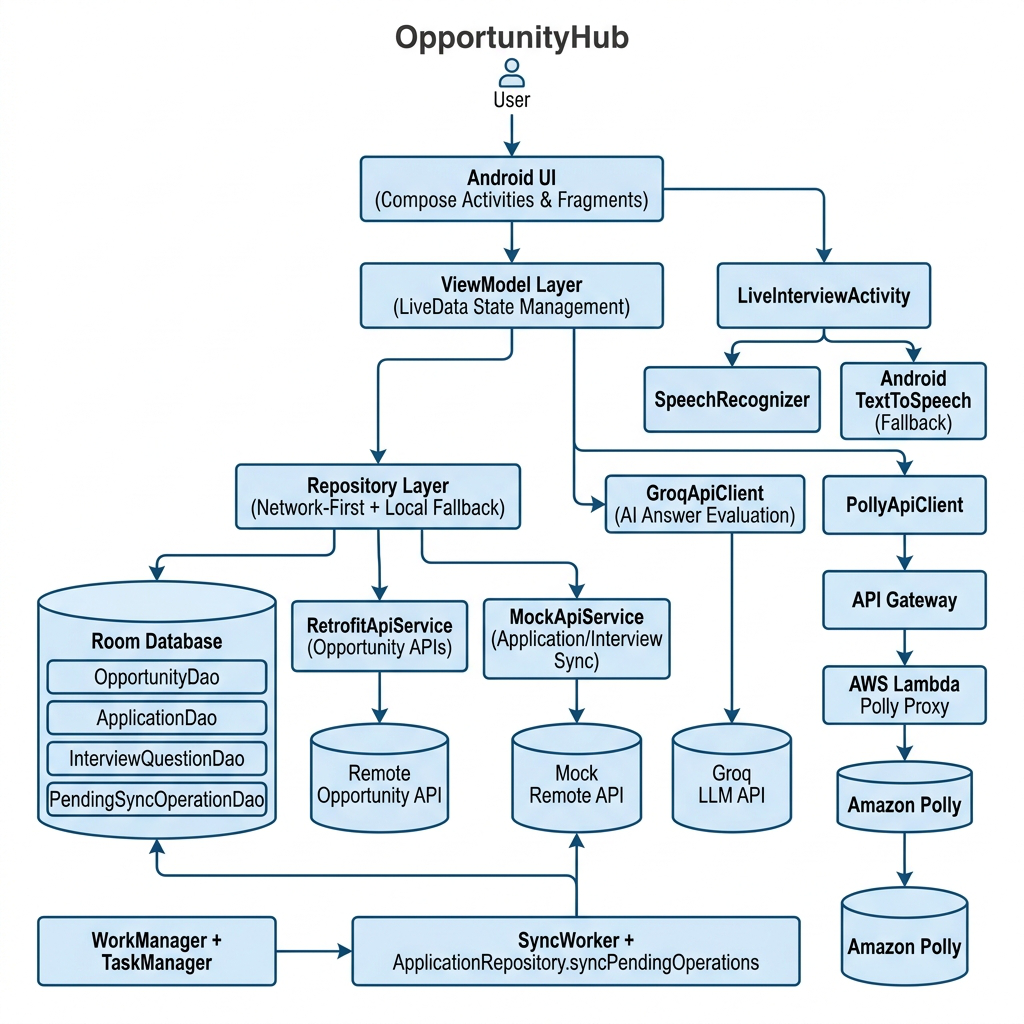
\includegraphics[width=0.98\textwidth]{report_assets/figures/figure_1.png}%
}{%
  \fbox{\parbox{0.9\textwidth}{Missing figure file: report\_assets/figures/figure\_1.png}}%
}
\caption{Fig. 1. 4.8.1 End-to-End Component Interaction}
\end{figure*}

\subsection{Sequence A: Opportunity Discovery Request/Response}

\begin{figure*}[!tb]
\centering
\IfFileExists{report_assets/figures/figure_2.png}{%
  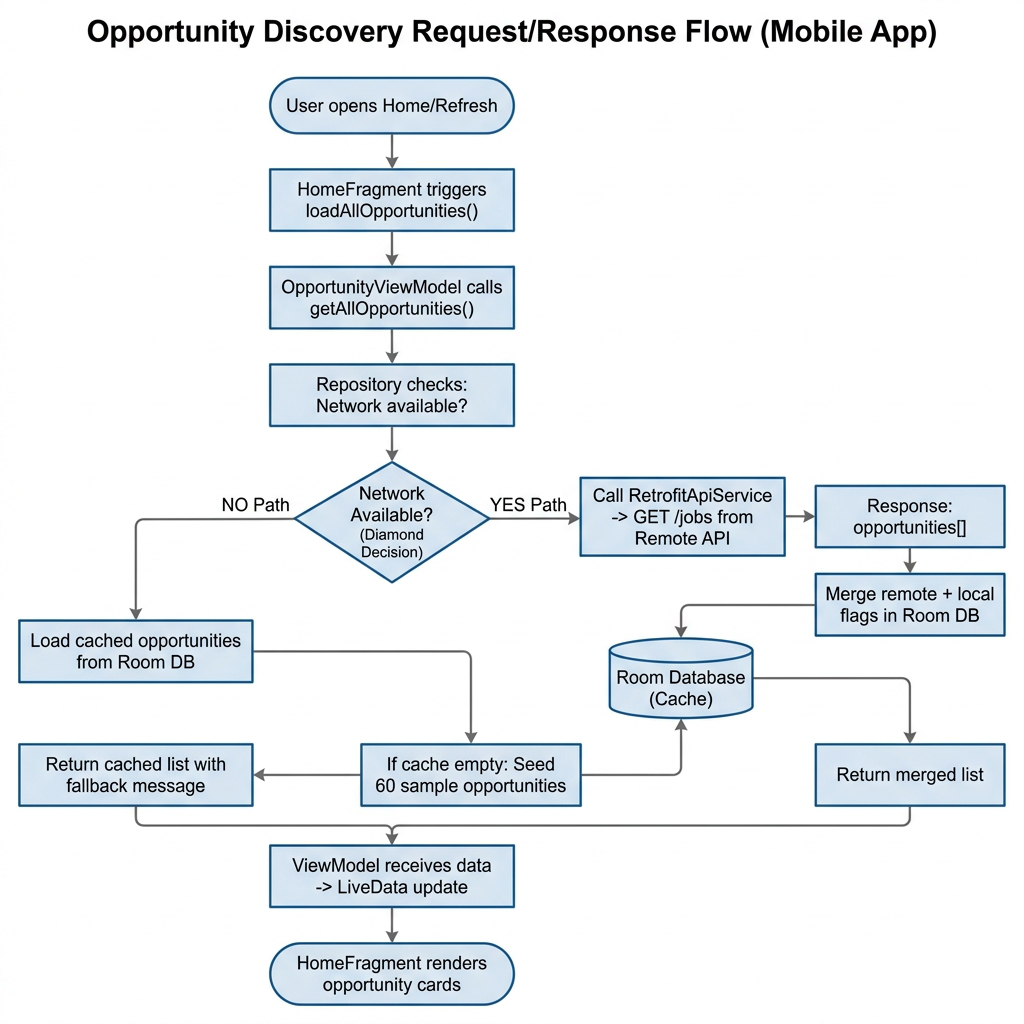
\includegraphics[width=0.98\textwidth]{report_assets/figures/figure_2.png}%
}{%
  \fbox{\parbox{0.9\textwidth}{Missing figure file: report\_assets/figures/figure\_2.png}}%
}
\caption{Fig. 2. 4.8.2 Sequence A: Opportunity Discovery Request/Response}
\end{figure*}

\subsection{Sequence B: Application Write + Offline Sync Queue}

\begin{figure*}[!tb]
\centering
\IfFileExists{report_assets/figures/figure_3.png}{%
  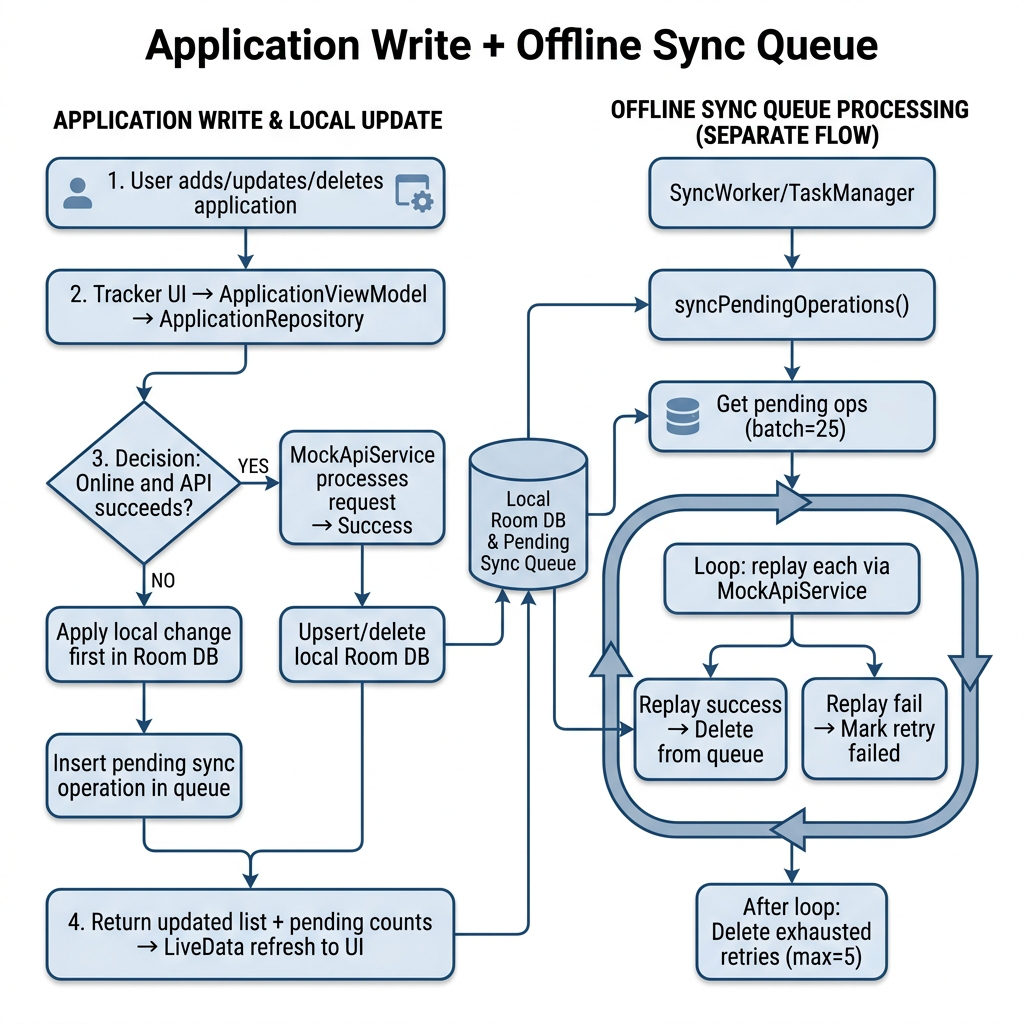
\includegraphics[width=0.98\textwidth]{report_assets/figures/figure_3.png}%
}{%
  \fbox{\parbox{0.9\textwidth}{Missing figure file: report\_assets/figures/figure\_3.png}}%
}
\caption{Fig. 3. 4.8.3 Sequence B: Application Write + Offline Sync Queue}
\end{figure*}

\subsection{Sequence C: AI Interview Evaluation (AI + Local Fallback)}

\begin{figure*}[!tb]
\centering
\IfFileExists{report_assets/figures/figure_4.png}{%
  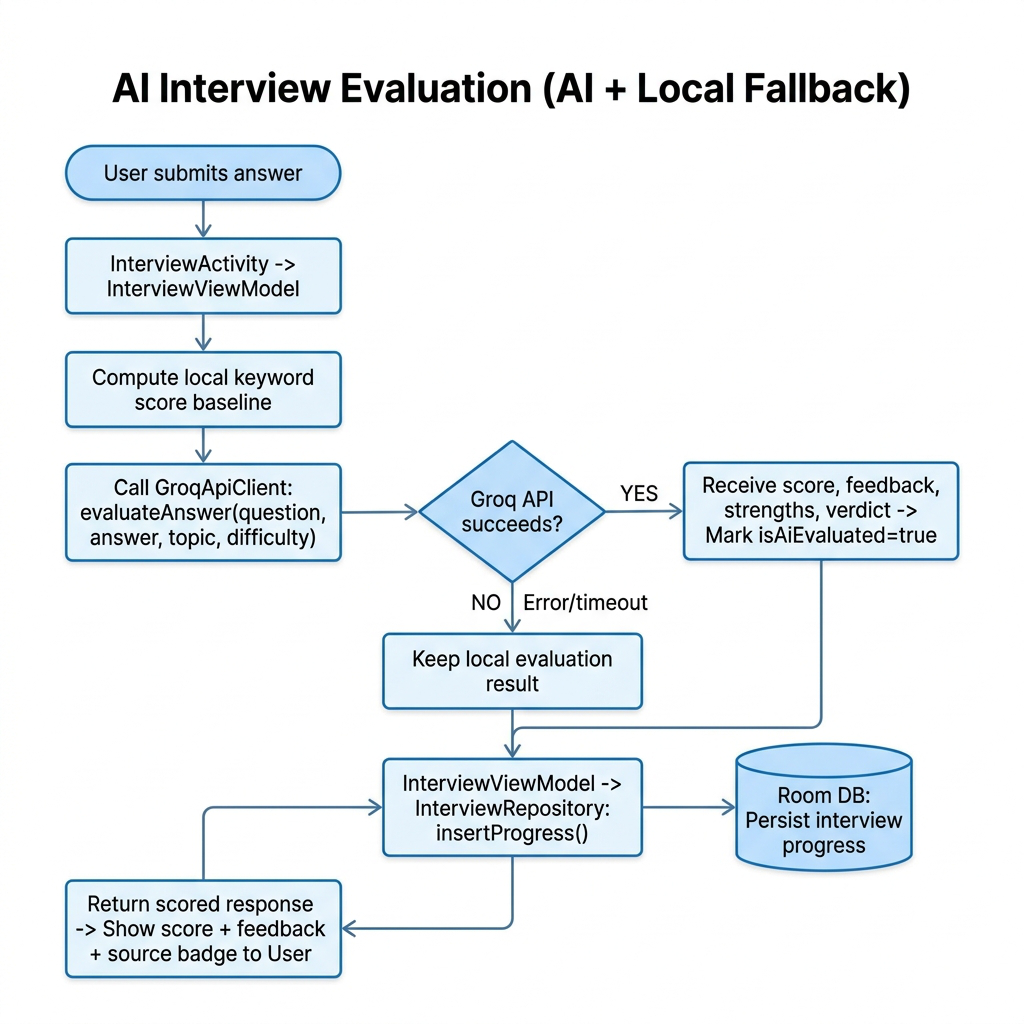
\includegraphics[width=0.98\textwidth]{report_assets/figures/figure_4.png}%
}{%
  \fbox{\parbox{0.9\textwidth}{Missing figure file: report\_assets/figures/figure\_4.png}}%
}
\caption{Fig. 4. 4.8.4 Sequence C: AI Interview Evaluation (AI + Local Fallback)}
\end{figure*}

\subsection{Sequence D: Live Interview Voice Loop (STT to Polly/TTS)}

\begin{figure*}[!tb]
\centering
\IfFileExists{report_assets/figures/figure_5.png}{%
  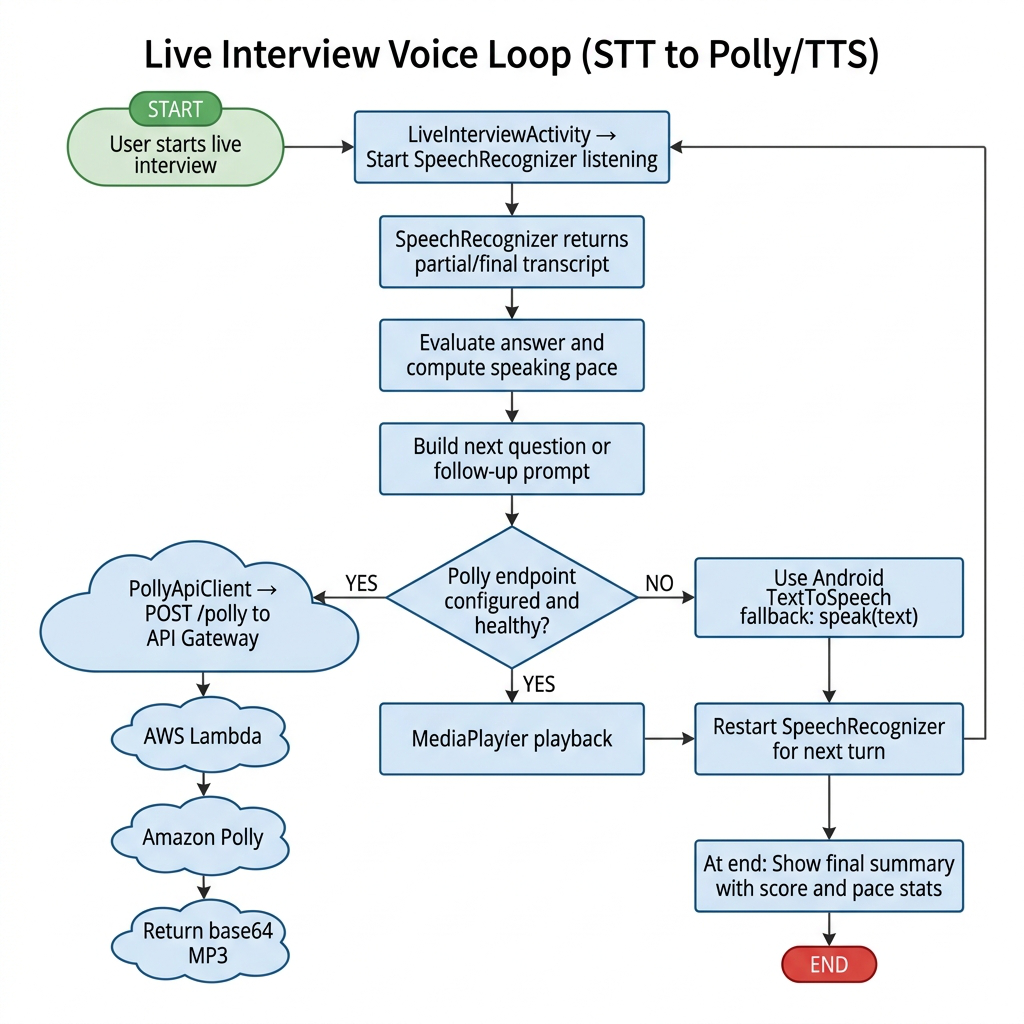
\includegraphics[width=0.98\textwidth]{report_assets/figures/figure_5.png}%
}{%
  \fbox{\parbox{0.9\textwidth}{Missing figure file: report\_assets/figures/figure\_5.png}}%
}
\caption{Fig. 5. 4.8.5 Sequence D: Live Interview Voice Loop (STT to Polly/TTS)}
\end{figure*}

\subsection{Request/Response Contract Snapshot}

\begin{table*}[!tb]
\centering
\setlength{\tabcolsep}{4pt}
\normalsize
\begin{tabularx}{\textwidth}{|>{\RaggedRight\arraybackslash}X|>{\RaggedRight\arraybackslash}X|>{\RaggedRight\arraybackslash}X|>{\RaggedRight\arraybackslash}X|}
\hline
 \textbf{Flow} & \textbf{Request} & \textbf{Response} & \textbf{Fallback Behavior} \\
\hline
 Opportunity fetch & GET opportunities via RetrofitApiService & List\textless{}Opportunity\textgreater{} & Load cached Room data; seed local sample if empty \\
\hline
 Application write & insert/update/delete application via MockApiService & success/fail callback & Write local first and enqueue pending\_sync\_operations \\
\hline
 Pending sync replay & batched replay of queued operations & per-op success/fail & increment retry count; remove after max retries \\
\hline
 Interview evaluation & evaluateAnswer(question, answer, topic, difficulty) via GroqApiClient & score, feedback, strengths, improvements, verdict & use local keyword-based evaluation \\
\hline
 Polly synthesis & POST /polly body: text, voiceId, engine, outputFormat & base64 MP3 audio (audio/mpeg) & fallback to Android TextToSpeech \\
\hline
\end{tabularx}
\end{table*}

These flows ensure a resilient mobile-first architecture where user-visible actions always produce timely local responses, even when remote services fail.

\subsection{API Endpoint Inventory}

This subsection lists the endpoint surface currently used by the application and classifies each endpoint by purpose, request shape, response contract, authentication model, and owning module.

\subsection{HTTP Endpoint Inventory (Implemented)}

\begin{table*}[!tb]
\centering
\setlength{\tabcolsep}{1.0pt}
\tiny
\begin{tabularx}{\textwidth}{|>{\RaggedRight\hspace{0pt}\arraybackslash}X|>{\RaggedRight\hspace{0pt}\arraybackslash}X|>{\RaggedRight\hspace{0pt}\arraybackslash}X|>{\RaggedRight\hspace{0pt}\arraybackslash}X|>{\RaggedRight\hspace{0pt}\arraybackslash}X|>{\RaggedRight\hspace{0pt}\arraybackslash}X|>{\RaggedRight\hspace{0pt}\arraybackslash}X|>{\RaggedRight\hspace{0pt}\arraybackslash}X|>{\RaggedRight\hspace{0pt}\arraybackslash}X|}
\hline
 \textbf{Endpoint ID} & \textbf{Base URL} & \textbf{Path} & \textbf{Method} & \textbf{Purpose} & \textbf{Request Contract} & \textbf{Response Contract} & \textbf{Auth} & \textbf{Consumed By} \\
\hline
 OPP-LIST-01 & \url{https://remotive.com} & /api/remote-jobs & GET & Fetch remote job opportunities and search results & Query params: limit (int), search (string, optional) & JSON with jobs[]; mapped to Opportunity model in app & None & \shortstack[l]{RetrofitApiService\\OpportunityRepository} \\
\hline
 AI-EVAL-01 & \url{https://api.groq.com} & \shortstack[l]{/openai/v1/chat/\\completions} & POST & Evaluate interview answers and stateful interview chat & \shortstack[l]{JSON body: model, messages[],\\max\_tokens, temperature} & \shortstack[l]{choices[0].message.content\\parsed to score/feedback/verdict} & Bearer token (GROQ\_API\_KEY) & \shortstack[l]{GroqApiClient\\InterviewViewModel} \\
\hline
 PLY-01 & endpoint & /polly & POST & Polly synthesis via proxy & \shortstack[l]{JSON: text, voiceId,\\engine, outputFormat} & \shortstack[l]{Base64 MP3 from\\Lambda proxy} & None (demo) & PollyClient \\
\hline
 PLY-02 & endpoint & /polly & OPTIONS & CORS preflight & No body & 200 with CORS headers & None & API GW \\
\hline
\end{tabularx}
\end{table*}

\subsection{Local Mock API Surface (Non-HTTP)}

The project also uses an in-process mock API service for development and offline simulation. These are API-like operations but do not expose network URLs.

\begin{table*}[!tb]
\centering
\setlength{\tabcolsep}{4pt}
\normalsize
\begin{tabularx}{\textwidth}{|>{\RaggedRight\arraybackslash}X|>{\RaggedRight\arraybackslash}X|>{\RaggedRight\arraybackslash}X|>{\RaggedRight\arraybackslash}X|}
\hline
 \textbf{Service} & \textbf{Operation} & \textbf{Transport Type} & \textbf{Current Role} \\
\hline
 MockApiService & fetchApplications, addApplication, updateApplication, deleteApplication & In-process method call & Simulated backend for application tracker write-through flow \\
\hline
 MockApiService & fetchQuestionsByDomain, fetchAllQuestions & In-process method call & Simulated interview question backend \\
\hline
 MockApiService & fetchUserStats & In-process method call & Simulated analytics summary backend \\
\hline
\end{tabularx}
\end{table*}

\subsection{Endpoint Readiness Notes}

Opportunity discovery is already backed by a real public HTTP endpoint (Remotive). AI interview scoring is already backed by a real LLM endpoint (Groq). Voice synthesis uses a configurable API Gateway + Lambda proxy endpoint for Amazon Polly. Application tracker and interview list sync currently rely on MockApiService. In production, these should be replaced with authenticated backend REST endpoints (for example, /applications, /interview/questions, /analytics/stats).

\section{Contribution Towards The Society And Environment}

\begin{itemize}
  \item \textbf{Career Accessibility:} Consolidates fragmented workflows, reducing cognitive and time burden for students and early professionals.
  \item \textbf{Skill Development:} Encourages structured interview practice with actionable feedback loops.
  \item \textbf{Inclusion Through Mobile-first Design:} Supports day-to-day use on common Android devices and intermittent connectivity.
  \item \textbf{Reduced Operational Waste:} Digital application tracking and reminders reduce dependence on ad-hoc manual note-taking and repeated effort.
  \item \textbf{Scalable Educational Utility:} The architecture can be reused in placement cells and institutional career support ecosystems.
\end{itemize}

\subsection{Low-Level Design (LLD)}

\begin{table*}[!tb]
\centering
\setlength{\tabcolsep}{4pt}
\normalsize
\begin{tabularx}{\textwidth}{|>{\RaggedRight\arraybackslash}X|>{\RaggedRight\arraybackslash}X|}
\hline
 \textbf{Module} & \textbf{Key Responsibilities} \\
\hline
 model & Entity/state definitions for opportunities, applications, interview, user profile \\
\hline
 database (Room + DAO) & Local CRUD, query filtering, pending sync storage \\
\hline
 repository & Network-first fetch, local fallback, sync-merge, write-through operations \\
\hline
 viewmodel & UI state orchestration, filtering, scoring, analytics aggregation \\
\hline
 ui/fragments + activities & User interactions, rendering, workflow control \\
\hline
 ai & Recommendation scoring, resume keyword extraction, interview evaluation logic \\
\hline
 worker & Background sync and notification routines \\
\hline
 util & Data generators, diagnostics, export, helpers \\
\hline
\end{tabularx}
\end{table*}

\subsection{High-Level Design (HLD)}

The application follows a layered pattern:

\begin{itemize}
  \item \textbf{Presentation Layer:} Compose screens for main workflows and interactions.
  \item \textbf{Domain/Logic Layer:} Recommendation and interview logic components.
  \item \textbf{Data Layer:} Repositories coordinating local+remote data strategy.
  \item \textbf{Persistence and Sync Layer:} Room entities, pending operation queues, periodic workers.
  \item \textbf{Device Integration Layer:} Speech recognition, TextToSpeech, CameraX, notification channels.
\end{itemize}

\section{Use Of Advanced Concepts}

\begin{itemize}
  \item MVVM architecture with reactive LiveData state propagation.
  \item Compose Material 3 UI with multi-screen state handling.
  \item Offline-first synchronization through queued pending operations and retry policies.
  \item WorkManager periodic jobs for sync and recommendations.
  \item Multi-factor recommendation and profile-aware scoring.
  \item Local and AI hybrid interview evaluation strategy.
  \item Live interview voice loop combining STT, adaptive prompting, and TTS/Polly output.
  \item CSV export for analytics portability.
  \item CameraX integration for real-time interview preview.
  \item SharedPreferences-driven personalization (theme, roadmap completion).
\end{itemize}

\section{Results And Discussions}

\subsection{Functional Results}

Table 1 summarizes feature-level implementation outcomes.

\begin{table*}[!tb]
\centering
\setlength{\tabcolsep}{4pt}
\normalsize
\begin{tabularx}{\textwidth}{|>{\RaggedRight\arraybackslash}X|>{\RaggedRight\arraybackslash}X|}
\hline
 \textbf{Feature Area} & \textbf{Implemented Outcome} \\
\hline
 Unified feed & Internship/job/hackathon listing with search and multi-chip filtering \\
\hline
 Recommendation & Profile-aware ranking and match percentage display \\
\hline
 Save/apply flow & Save toggling and applied-state transition from listing cards \\
\hline
 Tracker & Status filtering, edit/delete actions, sync-now control, pending sync visibility \\
\hline
 AI Interview & Domain selection, question loading, answer evaluation, session score flow \\
\hline
 Live Interview & Camera preview, speech capture, pace estimation, adaptive follow-up, spoken interviewer responses \\
\hline
 Analytics & Total/interview/offer metrics, success rate, readiness indicators, donut chart, CSV export \\
\hline
 Roadmap & Personalized roadmap generation and completion persistence \\
\hline
 Background automation & 15-minute sync worker + daily recommendation and deadline reminder workers \\
\hline
\end{tabularx}
\end{table*}

\subsection{Observed Quantitative/Configuration Evidence}

\begin{itemize}
  \item Recommendation output supports top-ranked subsets for UI and notifications.
  \item Local fallback seeding inserts 60 opportunities when no cache exists.
  \item Live interview plan uses a multi-turn structure (intro, technical set, probe, behavioral, closing).
  \item Sync system includes pending operation batching and retry control.
  \item Unit-test files exist for sync helper logic (application/opportunity/interview merge helpers).
\end{itemize}

\subsection{Build and Validation Discussion}

Project build behavior is environment-dependent due machine-specific SDK/JDK local paths. A prior build log in project artifacts indicates successful Gradle build in a properly configured environment. On the current machine, build validation was blocked by invalid local JDK/SDK path references.

\subsection{Discussion}

The project successfully demonstrates integration value: users can move from discovery to interview preparation without leaving the app context. The strongest practical contribution is the combination of profile-aware recommendations, resilient offline behavior, and live interview simulation. Compared to single-purpose tools, this integrated flow reduces context switching and supports continuity. The architecture is extensible for real APIs and institutional adoption.

\section{Conclusion}

OpportunityHub presents a comprehensive Android solution for opportunity lifecycle management. It unifies discovery, recommendation, tracking, analytics, and interview preparation in a coherent mobile system. The implementation combines modern Android architecture (MVVM, Room, WorkManager, Compose) with reliability-focused strategies (local fallback, queued sync, retry logic) and intelligent interaction features (AI evaluation and live voice interview flow). The project demonstrates that a mobile-first integrated platform can significantly improve consistency and readiness across the student career journey.

\section{Study Limitations}

\begin{itemize}
  \item Build reproducibility currently depends on correcting machine-specific local SDK/JDK paths.
  \item Resume parsing from raw PDF bytes is keyword-based and may miss structured PDF semantics.
  \item Some data flows still rely on mock API service behavior and need production API hardening.
  \item Default single-user assumptions (for example, fixed mock user ID) limit multi-user realism.
  \item Full-scale instrumented testing on diverse devices/emulators was constrained by environment configuration.
\end{itemize}

\section{Future Scope}

\begin{itemize}
  \item Integrate production opportunity APIs and authenticated user accounts.
  \item Add stronger resume parsing using robust document parsing pipelines.
  \item Extend recommendation with learning-to-rank, implicit feedback, and temporal modeling.
  \item Add richer interview analytics (topic weakness trajectories, confidence bands, adaptive sequencing).
  \item Expand roadmap generation with milestone deadlines and mentor feedback loops.
  \item Add CI/CD pipeline for automated unit/instrumented test execution.
  \item Improve privacy/security with encrypted local storage and finer-grained sync conflict strategies.
\end{itemize}

\FloatBarrier
\IEEEtriggeratref{19}
\begin{thebibliography}{99}
\small
\setlength{\itemsep}{0pt}
\setlength{\parskip}{0pt}
\setlength{\parsep}{0pt}
\bibitem{ref1} Android Developers, ``Guide to app architecture,'' [Online]. Available: \url{https://developer.android.com/topic/architecture}
\bibitem{ref2} Android Developers, ``WorkManager overview,'' [Online]. Available: \url{https://developer.android.com/topic/libraries/architecture/workmanager}
\bibitem{ref3} Android Developers, ``Room persistence library,'' [Online]. Available: \url{https://developer.android.com/training/data-storage/room}
\bibitem{ref4} Android Developers, ``CameraX architecture,'' [Online]. Available: \url{https://developer.android.com/media/camera/camerax}
\bibitem{ref5} Android Developers, ``SpeechRecognizer,'' [Online]. Available: \url{https://developer.android.com/reference/android/speech/SpeechRecognizer}
\bibitem{ref6} Android Developers, ``TextToSpeech,'' [Online]. Available: \url{https://developer.android.com/reference/android/speech/tts/TextToSpeech}
\bibitem{ref7} Android Developers, ``Jetpack Compose,'' [Online]. Available: \url{https://developer.android.com/jetpack/compose}
\bibitem{ref8} Square, ``Retrofit,'' [Online]. Available: \url{https://square.github.io/retrofit/}
\bibitem{ref9} Square, ``OkHttp,'' [Online]. Available: \url{https://square.github.io/okhttp/}
\bibitem{ref10} Google, ``Material Design 3,'' [Online]. Available: \url{https://m3.material.io/}
\bibitem{ref11} Amazon Web Services, ``Amazon Polly Developer Guide,'' [Online]. Available: \url{https://docs.aws.amazon.com/polly/}
\bibitem{ref12} LinkedIn, ``Jobs on LinkedIn,'' [Online]. Available: \url{https://www.linkedin.com/jobs/}
\bibitem{ref13} Indeed, ``Job Search,'' [Online]. Available: \url{https://www.indeed.com/}
\bibitem{ref14} LeetCode, ``Interview preparation resources,'' [Online]. Available: \url{https://leetcode.com/}
\bibitem{ref15} HackerRank, ``Technical skill practice platform,'' [Online]. Available: \url{https://www.hackerrank.com/}
\bibitem{ref16} Devpost, ``Hackathon platform,'' [Online]. Available: \url{https://devpost.com/}
\bibitem{ref17} HackerEarth, ``Hackathons and developer assessments,'' [Online]. Available: \url{https://www.hackerearth.com/}
\bibitem{ref18} Firebase, ``Authentication and cloud services documentation,'' [Online]. Available: \url{https://firebase.google.com/docs}
\bibitem{ref19} M. Fowler, ``Microservices,'' [Online]. Available: \url{https://martinfowler.com/articles/microservices.html}
\bibitem{ref20} IEEE Xplore, ``Mobile and cloud software reliability studies,'' [Online]. Available: \url{https://ieeexplore.ieee.org/}
\bibitem{ref21} G. Adomavicius and A. Tuzhilin, ``Toward the Next Generation of Recommender Systems: A Survey of the State-of-the-Art and Possible Extensions,'' \emph{IEEE Transactions on Knowledge and Data Engineering}, vol. 17, no. 6, pp. 734--749, 2005.
\bibitem{ref22} R. Burke, ``Hybrid Recommender Systems: Survey and Experiments,'' \emph{User Modeling and User-Adapted Interaction}, vol. 12, no. 4, pp. 331--370, 2002.
\bibitem{ref23} Y. Koren, R. Bell, and C. Volinsky, ``Matrix Factorization Techniques for Recommender Systems,'' \emph{Computer}, vol. 42, no. 8, pp. 30--37, 2009.
\bibitem{ref24} T. Burrows, I. Gurevych, and B. Stein, ``The Eras and Trends of Automatic Short Answer Grading,'' \emph{International Journal of Artificial Intelligence in Education}, vol. 25, no. 1, pp. 60--117, 2015.
\bibitem{ref25} A. Vaswani \emph{et al.}, ``Attention Is All You Need,'' in \emph{Advances in Neural Information Processing Systems (NeurIPS)}, pp. 5998--6008, 2017.
\bibitem{ref26} J. Devlin, M.-W. Chang, K. Lee, and K. Toutanova, ``BERT: Pre-training of Deep Bidirectional Transformers for Language Understanding,'' in \emph{Proc. NAACL-HLT}, pp. 4171--4186, 2019.

\end{thebibliography}

\end{document}